%!TEX root=../report.tex

\section{Example: Model Card Games as Discrete-Event Simulation}


I focus on card games as examples. The focus on card games is due to the wide range of different types of board games. Board games, in general, are too diverse in terms of materials (game board, cards, meeples) and rules. In contrast to that, most card games share the same game elements. To be even more specific, the implementation mainly addresses shedding games, like \textit{UNO}, \textit{The Great Dalmuti} and \textit{Phase 10} \cite{wiki:sheddinglist}. They have at least one discard pile, where all players contribute to. They have a hand for each player and optionally shared or not shared open played cards. Additionally, they may have a draw pile. Cards consist of color or a symbol, a number, and maybe a special rule is attached to them.
The game rules of card games are that all players take their turn one after the other. There is no concurrency. This excludes some card games that aim for competing in reaction time, but this is not the scope of this implementation.

The decision to build a framework from scratch was derived from the specific conditions that card games have.
In the next section, I will explain my implementation, followed by a concrete implementation of the card game \uno.

The objective of the implementation is to build a framework that

\begin{itemize}
\item maps all main components of discrete-event simulation to the context of card games
\item uses an object-oriented approach for intuitive readability
\item is generic enough to cover common card games
\item keeps the implementation effort low for new player behavior and new games
\end{itemize}

The code is written in Python and published on GitHub at \url{https://github.com/paszin/card-game-simulation}.

\subsection{Data Structures}


All piles are implemented with the data structure of stacks. In computer science, a stack is a collection of data in which data can be inserted or deleted only at the top of the stack. \cite[page 86]{patel2018data}
Stacks implement the functions of push (add data at the top) and pop (delete data at the top).

Cards are the main data objects. They have the read only attributes \textit{color} and \textit{number} along with one writeable attribute \textit{valid}.
The Attribute \textit{valid} is used to save the information if the effect of the card was already applied.

% \note{Gamestate follows flux pattern}

\subsection{Simulation Logic}


There are some main components that a discrete event simulation requires.
This follows up on the components introduced in \ref{des:components}. I will explain how I implemented the components in my card game framework.
The overall execution logic of the simulations follows the concepts of next-event simulation in \ref{des:nextevent}.

\begin{description}
\item[System State] This captures all variables that characterize the simulation. In my case, the system state consists of the number of the current turn, the discard pile, the draw pile, and the hand of the players.

\item[Simulation Clock] This is a tool that tracks the elapsed time. For card games, the simulation clock is a counter of the turns. It gets incremented every time a player starts its turn. The initial value is zero. The simulation clock uses a fixed-increment advance. The turn-counter always increments by one and no interruptions by other players are possible. As interruptions are uncommon for card games, the simulation clock acts similar to a next-event time-advance, because the turn counter only increments, if the next player has a turn. The only accepted interruptions are triggered by the current player or other game objects like the draw pile. An exception handler is able to handle the exception. One exception is the end of the game, which is handled by breaking out of the simulation loop.

\item[Next-Event List] This is a queue of the upcoming events. For games, events are equal to making a turn. In my implementation, the next event is defined by a function that returns the next player. The choice of which player comes next depends on the current system state.

\item[Statistical Counter or Accumulator] This is a tool that records the evolution of the system state. My implementation saves a copy of the current system state after each turn. From this list of game states, a specific development of one variable can be derived.

\end{description}

\begin{figure}[h!]
\caption{Overview of objects, its methods and pseudo-code of simulation function}
\centering
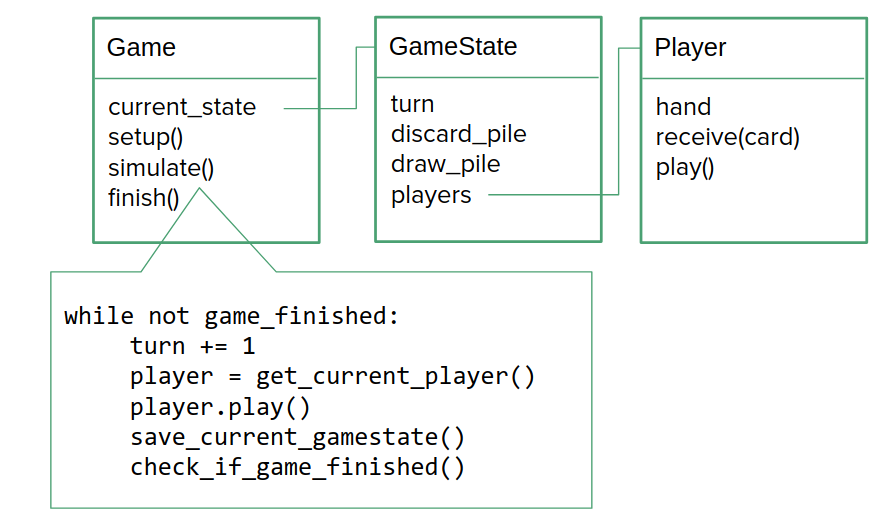
\includegraphics[width=0.8\textwidth]{class-diagram}
\label{fig:class-diagram}
\end{figure}

%
%The initialization program is the setup method of the game class.
%
%
%The event subprogram is in the simulate function of the game class. In pseudo-code the simulate function runs in a loop till the game is finished. And we call the player.play function that modifies the current game state. This function contains all the logic to play the game. In my implementation it’s pick a card with the same color or same number otherwise take a card from the draw pile.
%
%The event subprogram is in the simulate function of the game class. In pseudo code the simulate functions runs in a loop till the game is finished. And we call the player.play function that modifies the current game state. This function contains all the logic to play the game. In my implementation it’s pick a card with the same color or same number otherwise take a card from the draw pile
%.

%
%(5) Initialization Subprogram. A protocol utilized in the initialization of
%the simulation, usually setting the start time to zero.
%(6) Timing Subprogram. A protocol that, drawing from a next - event list,
%sets the next event and progresses the simulation clock to the moment
%when an event is to happen.
%(7) Event Subprogram. A protocol that launches a routine that updates
%the state of the system with the occurrence of each event.
%(8) Library Subprogram. A protocol used to produce random observa-
%tions drawn generally from predetermined probability distributions.
%(9) Report Generator. A tool that calculates and reports statistics that
%describe the performance of the system.
%(10) Main Program. A routine that coordinates the concert of subordinate
%routines, executing these in the correct sequence. It initializes the
%timing subprogram that determines the subsequent event, passes
%control to the related event subprogram, and updates the system state.
%This routine verifi es for termination and triggers the report generator
%once the simulation ends.



\subsection{Implementation of Uno}

As a first example, I will introduce \uno. In \uno, every player gets seven cards. The rest of the cards are placed face down on a draw pile. Next to the pile is a discard pile. The top card should be placed on the discard pile and the game begins. The players make their turns one after each other. A player could either put a card on the discard pile if it matches the last card or draws a card until one player has no more cards. Some special cards could have an effect on how the game evolves. Janssen derived eleven rule variations for \uno\ by comparing it to \textit{Crazy Eights} for his studies \cite{janssen2010evolution}.

At first, I implement a simplified version of \uno. My \textit{simplified UNO}  drops all special cards. The idea of the modification is that this is still a good abstraction to simulate the flow of \uno. Furthermore, observations of this version of the game can be used as an indicator of whether there is a need for special cards that make the game more difficult or easier. Special cards could be added sequentially to measure the impact of a new card. Without special cards, the card deck consists of the cards one to nine, two times in four different colors.

To extend the framework I have to implement derived classes from the \textit{Game}-class and the \textit{Player}-class. The new \textit{Game}-class must implement the \textit{setup}-method and the new \textit{Player}-class must implement the \textit{play}-method.

The implementation of the \textit{setup}-method must start with the generation of the card deck. This is done by nested for-loops over the colors and numbers of the deck. The last step is setting the game state. Inbetween the \textit{setup}-method follows the game instruction of \uno. To extend this, special cards can be added to the card deck.

The player behavior is implemented as choosing the first card that could be put on the discard pile. The first card means the card that holds the player for the longest time. This results in a deterministic turn. 
\newpage
The advanced version the player behavior follows these steps:

\begin{itemize}
\item[1.] Check if the last card on the discard pile expects any special considerations.
\item[2.] Filter all cards that could be put on the discard pile.
\item[3.] Rate the cards. Special cards get a higher rating.
\item[4.] Chose the card with the lowest rating.
\end{itemize}

The intention of the player behavior is to avoid playing wild cards without the need to change the color and to keep other special cards for the end game. This player behavior is derived from personal observations. Different player types could be implemented that play special cards more aggressively. Also, interactive player types are possible. The \textit{play}-method could depend on the input by a user.







